\documentclass[1p]{elsarticle_modified}
%\bibliographystyle{elsarticle-num}

%\usepackage[colorlinks]{hyperref}
%\usepackage{abbrmath_seonhwa} %\Abb, \Ascr, \Acal ,\Abf, \Afrak
\usepackage{amsfonts}
\usepackage{amssymb}
\usepackage{amsmath}
\usepackage{amsthm}
\usepackage{scalefnt}
\usepackage{amsbsy}
\usepackage{kotex}
\usepackage{caption}
\usepackage{subfig}
\usepackage{color}
\usepackage{graphicx}
\usepackage{xcolor} %% white, black, red, green, blue, cyan, magenta, yellow
\usepackage{float}
\usepackage{setspace}
\usepackage{hyperref}

\usepackage{tikz}
\usetikzlibrary{arrows}

\usepackage{multirow}
\usepackage{array} % fixed length table
\usepackage{hhline}

%%%%%%%%%%%%%%%%%%%%%
\makeatletter
\renewcommand*\env@matrix[1][\arraystretch]{%
	\edef\arraystretch{#1}%
	\hskip -\arraycolsep
	\let\@ifnextchar\new@ifnextchar
	\array{*\c@MaxMatrixCols c}}
\makeatother %https://tex.stackexchange.com/questions/14071/how-can-i-increase-the-line-spacing-in-a-matrix
%%%%%%%%%%%%%%%

\usepackage[normalem]{ulem}

\newcommand{\msout}[1]{\ifmmode\text{\sout{\ensuremath{#1}}}\else\sout{#1}\fi}
%SOURCE: \msout is \stkout macro in https://tex.stackexchange.com/questions/20609/strikeout-in-math-mode

\newcommand{\cancel}[1]{
	\ifmmode
	{\color{red}\msout{#1}}
	\else
	{\color{red}\sout{#1}}
	\fi
}

\newcommand{\add}[1]{
	{\color{blue}\uwave{#1}}
}

\newcommand{\replace}[2]{
	\ifmmode
	{\color{red}\msout{#1}}{\color{blue}\uwave{#2}}
	\else
	{\color{red}\sout{#1}}{\color{blue}\uwave{#2}}
	\fi
}

\newcommand{\Sol}{\mathcal{S}} %segment
\newcommand{\D}{D} %diagram
\newcommand{\A}{\mathcal{A}} %arc


%%%%%%%%%%%%%%%%%%%%%%%%%%%%%5 test

\def\sl{\operatorname{\textup{SL}}(2,\Cbb)}
\def\psl{\operatorname{\textup{PSL}}(2,\Cbb)}
\def\quan{\mkern 1mu \triangleright \mkern 1mu}

\theoremstyle{definition}
\newtheorem{thm}{Theorem}[section]
\newtheorem{prop}[thm]{Proposition}
\newtheorem{lem}[thm]{Lemma}
\newtheorem{ques}[thm]{Question}
\newtheorem{cor}[thm]{Corollary}
\newtheorem{defn}[thm]{Definition}
\newtheorem{exam}[thm]{Example}
\newtheorem{rmk}[thm]{Remark}
\newtheorem{alg}[thm]{Algorithm}

\newcommand{\I}{\sqrt{-1}}
\begin{document}

%\begin{frontmatter}
%
%\title{Boundary parabolic representations of knots up to 8 crossings}
%
%%% Group authors per affiliation:
%\author{Yunhi Cho} 
%\address{Department of Mathematics, University of Seoul, Seoul, Korea}
%\ead{yhcho@uos.ac.kr}
%
%
%\author{Seonhwa Kim} %\fnref{s_kim}}
%\address{Center for Geometry and Physics, Institute for Basic Science, Pohang, 37673, Korea}
%\ead{ryeona17@ibs.re.kr}
%
%\author{Hyuk Kim}
%\address{Department of Mathematical Sciences, Seoul National University, Seoul 08826, Korea}
%\ead{hyukkim@snu.ac.kr}
%
%\author{Seokbeom Yoon}
%\address{Department of Mathematical Sciences, Seoul National University, Seoul, 08826,  Korea}
%\ead{sbyoon15@snu.ac.kr}
%
%\begin{abstract}
%We find all boundary parabolic representation of knots up to 8 crossings.
%
%\end{abstract}
%\begin{keyword}
%    \MSC[2010] 57M25 
%\end{keyword}
%
%\end{frontmatter}

%\linenumbers
%\tableofcontents
%
\newcommand\colored[1]{\textcolor{white}{\rule[-0.35ex]{0.8em}{1.4ex}}\kern-0.8em\color{red} #1}%
%\newcommand\colored[1]{\textcolor{white}{ #1}\kern-2.17ex	\textcolor{white}{ #1}\kern-1.81ex	\textcolor{white}{ #1}\kern-2.15ex\color{red}#1	}

{\Large $\underline{12a_{1170}~(K12a_{1170})}$}

\setlength{\tabcolsep}{10pt}
\renewcommand{\arraystretch}{1.6}
\vspace{1cm}\begin{tabular}{m{100pt}>{\centering\arraybackslash}m{274pt}}
\multirow{5}{120pt}{
	\centering
	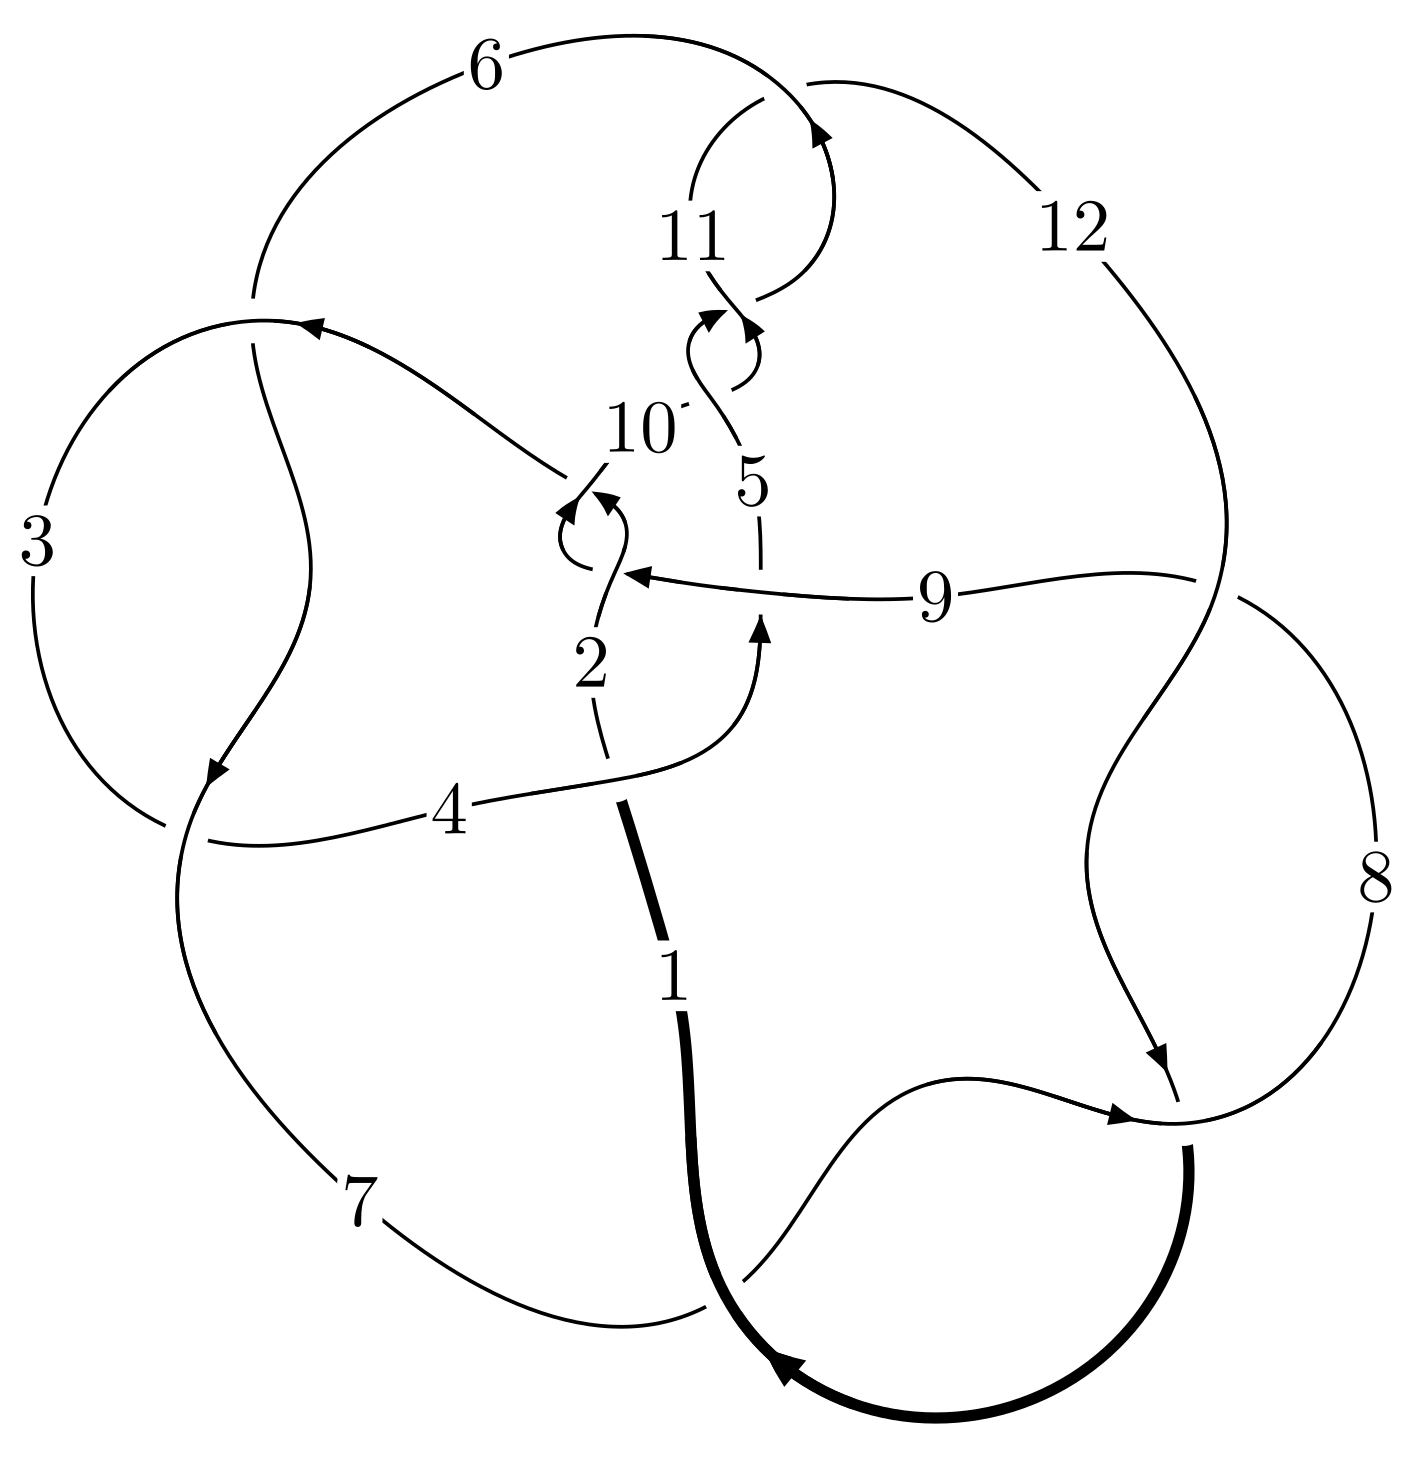
\includegraphics[width=112pt]{../../../GIT/diagram.site/Diagrams/png/1971_12a_1170.png}\\
\ \ \ A knot diagram\footnotemark}&
\allowdisplaybreaks
\textbf{Linearized knot diagam} \\
\cline{2-2}
 &
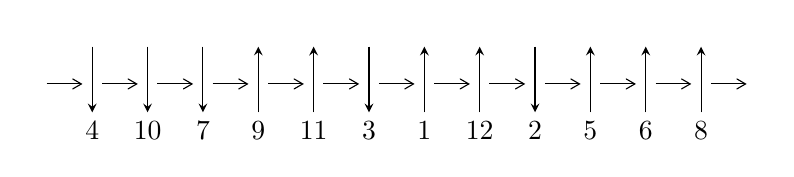
\begin{tikzpicture}[x=20pt, y=17pt]
	% nodes
	\node (C0) at (0, 0) {};
	\node (C1) at (1, 0) {};
	\node (C1U) at (1, +1) {};
	\node (C1D) at (1, -1) {4};

	\node (C2) at (2, 0) {};
	\node (C2U) at (2, +1) {};
	\node (C2D) at (2, -1) {10};

	\node (C3) at (3, 0) {};
	\node (C3U) at (3, +1) {};
	\node (C3D) at (3, -1) {7};

	\node (C4) at (4, 0) {};
	\node (C4U) at (4, +1) {};
	\node (C4D) at (4, -1) {9};

	\node (C5) at (5, 0) {};
	\node (C5U) at (5, +1) {};
	\node (C5D) at (5, -1) {11};

	\node (C6) at (6, 0) {};
	\node (C6U) at (6, +1) {};
	\node (C6D) at (6, -1) {3};

	\node (C7) at (7, 0) {};
	\node (C7U) at (7, +1) {};
	\node (C7D) at (7, -1) {1};

	\node (C8) at (8, 0) {};
	\node (C8U) at (8, +1) {};
	\node (C8D) at (8, -1) {12};

	\node (C9) at (9, 0) {};
	\node (C9U) at (9, +1) {};
	\node (C9D) at (9, -1) {2};

	\node (C10) at (10, 0) {};
	\node (C10U) at (10, +1) {};
	\node (C10D) at (10, -1) {5};

	\node (C11) at (11, 0) {};
	\node (C11U) at (11, +1) {};
	\node (C11D) at (11, -1) {6};

	\node (C12) at (12, 0) {};
	\node (C12U) at (12, +1) {};
	\node (C12D) at (12, -1) {8};
	\node (C13) at (13, 0) {};

	% arrows
	\draw[->,>={angle 60}]
	(C0) edge (C1) (C1) edge (C2) (C2) edge (C3) (C3) edge (C4) (C4) edge (C5) (C5) edge (C6) (C6) edge (C7) (C7) edge (C8) (C8) edge (C9) (C9) edge (C10) (C10) edge (C11) (C11) edge (C12) (C12) edge (C13) ;	\draw[->,>=stealth]
	(C1U) edge (C1D) (C2U) edge (C2D) (C3U) edge (C3D) (C4D) edge (C4U) (C5D) edge (C5U) (C6U) edge (C6D) (C7D) edge (C7U) (C8D) edge (C8U) (C9U) edge (C9D) (C10D) edge (C10U) (C11D) edge (C11U) (C12D) edge (C12U) ;
	\end{tikzpicture} \\
\hhline{~~} \\& 
\textbf{Solving Sequence} \\ \cline{2-2} 
 &
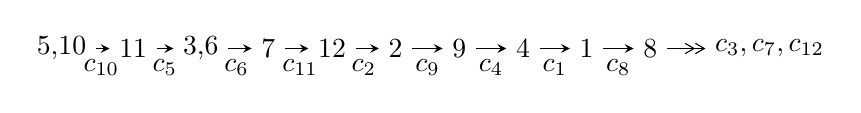
\begin{tikzpicture}[x=23pt, y=7pt]
	% node
	\node (A0) at (-1/8, 0) {5,10};
	\node (A1) at (1, 0) {11};
	\node (A2) at (33/16, 0) {3,6};
	\node (A3) at (25/8, 0) {7};
	\node (A4) at (33/8, 0) {12};
	\node (A5) at (41/8, 0) {2};
	\node (A6) at (49/8, 0) {9};
	\node (A7) at (57/8, 0) {4};
	\node (A8) at (65/8, 0) {1};
	\node (A9) at (73/8, 0) {8};
	\node (C1) at (1/2, -1) {$c_{10}$};
	\node (C2) at (3/2, -1) {$c_{5}$};
	\node (C3) at (21/8, -1) {$c_{6}$};
	\node (C4) at (29/8, -1) {$c_{11}$};
	\node (C5) at (37/8, -1) {$c_{2}$};
	\node (C6) at (45/8, -1) {$c_{9}$};
	\node (C7) at (53/8, -1) {$c_{4}$};
	\node (C8) at (61/8, -1) {$c_{1}$};
	\node (C9) at (69/8, -1) {$c_{8}$};
	\node (A10) at (11, 0) {$c_{3},c_{7},c_{12}$};

	% edge
	\draw[->,>=stealth]	
	(A0) edge (A1) (A1) edge (A2) (A2) edge (A3) (A3) edge (A4) (A4) edge (A5) (A5) edge (A6) (A6) edge (A7) (A7) edge (A8) (A8) edge (A9) ;
	\draw[->>,>={angle 60}]	
	(A9) edge (A10);
\end{tikzpicture} \\ 

\end{tabular} \\

\footnotetext{
The image of knot diagram is generated by the software ``\textbf{Draw programme}" developed by Andrew Bartholomew(\url{http://www.layer8.co.uk/maths/draw/index.htm\#Running-draw}), where we modified some parts for our purpose(\url{https://github.com/CATsTAILs/LinksPainter}).
}\phantom \\ \newline 
\centering \textbf{Ideals for irreducible components\footnotemark of $X_{\text{par}}$} 
 
\begin{align*}
I^u_{1}&=\langle 
4.42559\times10^{207} u^{102}-2.50511\times10^{206} u^{101}+\cdots+7.24447\times10^{208} b-6.34599\times10^{209},\\
\phantom{I^u_{1}}&\phantom{= \langle  }-3.30509\times10^{211} u^{102}+6.96912\times10^{210} u^{101}+\cdots+1.25329\times10^{211} a+5.02027\times10^{213},\\
\phantom{I^u_{1}}&\phantom{= \langle  }u^{103}+u^{102}+\cdots+988 u-173\rangle \\
I^u_{2}&=\langle 
-14120 u^{26}+4722 u^{25}+\cdots+7787 b-8083,\;18524 u^{26}+2179 u^{25}+\cdots+7787 a-2475,\\
\phantom{I^u_{2}}&\phantom{= \langle  }u^{27}-14 u^{25}+\cdots+4 u^2+1\rangle \\
\\
\end{align*}
\raggedright * 2 irreducible components of $\dim_{\mathbb{C}}=0$, with total 130 representations.\\
\footnotetext{All coefficients of polynomials are rational numbers. But the coefficients are sometimes approximated in decimal forms when there is not enough margin.}
\newpage
\renewcommand{\arraystretch}{1}
\centering \section*{I. $I^u_{1}= \langle 4.43\times10^{207} u^{102}-2.51\times10^{206} u^{101}+\cdots+7.24\times10^{208} b-6.35\times10^{209},\;-3.31\times10^{211} u^{102}+6.97\times10^{210} u^{101}+\cdots+1.25\times10^{211} a+5.02\times10^{213},\;u^{103}+u^{102}+\cdots+988 u-173 \rangle$}
\flushleft \textbf{(i) Arc colorings}\\
\begin{tabular}{m{7pt} m{180pt} m{7pt} m{180pt} }
\flushright $a_{5}=$&$\begin{pmatrix}0\\u\end{pmatrix}$ \\
\flushright $a_{10}=$&$\begin{pmatrix}1\\0\end{pmatrix}$ \\
\flushright $a_{11}=$&$\begin{pmatrix}1\\- u^2\end{pmatrix}$ \\
\flushright $a_{3}=$&$\begin{pmatrix}2.63712 u^{102}-0.556064 u^{101}+\cdots+2614.38 u-400.566\\-0.0610892 u^{102}+0.00345796 u^{101}+\cdots-49.6740 u+8.75976\end{pmatrix}$ \\
\flushright $a_{6}=$&$\begin{pmatrix}u\\- u^3+u\end{pmatrix}$ \\
\flushright $a_{7}=$&$\begin{pmatrix}3.52331 u^{102}-0.839955 u^{101}+\cdots+3545.53 u-544.506\\0.762710 u^{102}-0.270469 u^{101}+\cdots+839.144 u-128.842\end{pmatrix}$ \\
\flushright $a_{12}=$&$\begin{pmatrix}- u^2+1\\u^4-2 u^2\end{pmatrix}$ \\
\flushright $a_{2}=$&$\begin{pmatrix}2.57603 u^{102}-0.552606 u^{101}+\cdots+2564.71 u-391.806\\-0.0610892 u^{102}+0.00345796 u^{101}+\cdots-49.6740 u+8.75976\end{pmatrix}$ \\
\flushright $a_{9}=$&$\begin{pmatrix}2.21085 u^{102}-0.181129 u^{101}+\cdots+1993.54 u-299.459\\-0.120933 u^{102}+0.117634 u^{101}+\cdots-172.565 u+26.1483\end{pmatrix}$ \\
\flushright $a_{4}=$&$\begin{pmatrix}-1.00730 u^{102}+0.411475 u^{101}+\cdots-1126.72 u+174.496\\-1.64707 u^{102}+0.609439 u^{101}+\cdots-1807.03 u+281.022\end{pmatrix}$ \\
\flushright $a_{1}=$&$\begin{pmatrix}0.0593670 u^{102}-0.0345648 u^{101}+\cdots+33.9575 u-4.09273\\1.01418 u^{102}-0.128591 u^{101}+\cdots+934.610 u-140.366\end{pmatrix}$ \\
\flushright $a_{8}=$&$\begin{pmatrix}2.90932 u^{102}-0.278749 u^{101}+\cdots+2654.63 u-398.843\\1.52886 u^{102}-0.105690 u^{101}+\cdots+1374.19 u-208.465\end{pmatrix}$\\&\end{tabular}
\flushleft \textbf{(ii) Obstruction class $= -1$}\\~\\
\flushleft \textbf{(iii) Cusp Shapes $= -2.09664 u^{102}+0.747844 u^{101}+\cdots-2298.53 u+369.408$}\\~\\
\newpage\renewcommand{\arraystretch}{1}
\flushleft \textbf{(iv) u-Polynomials at the component}\newline \\
\begin{tabular}{m{50pt}|m{274pt}}
Crossings & \hspace{64pt}u-Polynomials at each crossing \\
\hline $$\begin{aligned}c_{1}\end{aligned}$$&$\begin{aligned}
&u^{103}-4 u^{102}+\cdots+63177613 u-8582393
\end{aligned}$\\
\hline $$\begin{aligned}c_{2},c_{9}\end{aligned}$$&$\begin{aligned}
&u^{103}- u^{102}+\cdots+1650 u+121
\end{aligned}$\\
\hline $$\begin{aligned}c_{3},c_{6}\end{aligned}$$&$\begin{aligned}
&u^{103}-43 u^{101}+\cdots+295139 u+37247
\end{aligned}$\\
\hline $$\begin{aligned}c_{4}\end{aligned}$$&$\begin{aligned}
&u^{103}+3 u^{102}+\cdots-1835136 u-186624
\end{aligned}$\\
\hline $$\begin{aligned}c_{5},c_{10},c_{11}\end{aligned}$$&$\begin{aligned}
&u^{103}- u^{102}+\cdots+988 u+173
\end{aligned}$\\
\hline $$\begin{aligned}c_{7},c_{8},c_{12}\end{aligned}$$&$\begin{aligned}
&u^{103}-2 u^{102}+\cdots-30 u-1
\end{aligned}$\\
\hline
\end{tabular}\\~\\
\newpage\renewcommand{\arraystretch}{1}
\flushleft \textbf{(v) Riley Polynomials at the component}\newline \\
\begin{tabular}{m{50pt}|m{274pt}}
Crossings & \hspace{64pt}Riley Polynomials at each crossing \\
\hline $$\begin{aligned}c_{1}\end{aligned}$$&$\begin{aligned}
&y^{103}-52 y^{102}+\cdots+1577684931052899 y-73657469606449
\end{aligned}$\\
\hline $$\begin{aligned}c_{2},c_{9}\end{aligned}$$&$\begin{aligned}
&y^{103}-65 y^{102}+\cdots+1848880 y-14641
\end{aligned}$\\
\hline $$\begin{aligned}c_{3},c_{6}\end{aligned}$$&$\begin{aligned}
&y^{103}-86 y^{102}+\cdots+48391156629 y-1387339009
\end{aligned}$\\
\hline $$\begin{aligned}c_{4}\end{aligned}$$&$\begin{aligned}
&y^{103}+17 y^{102}+\cdots-8707129344 y-34828517376
\end{aligned}$\\
\hline $$\begin{aligned}c_{5},c_{10},c_{11}\end{aligned}$$&$\begin{aligned}
&y^{103}-95 y^{102}+\cdots+361302 y-29929
\end{aligned}$\\
\hline $$\begin{aligned}c_{7},c_{8},c_{12}\end{aligned}$$&$\begin{aligned}
&y^{103}+108 y^{102}+\cdots+550 y-1
\end{aligned}$\\
\hline
\end{tabular}\\~\\
\newpage\flushleft \textbf{(vi) Complex Volumes and Cusp Shapes}
$$\begin{array}{c|c|c}  
\text{Solutions to }I^u_{1}& \I (\text{vol} + \sqrt{-1}CS) & \text{Cusp shape}\\
 \hline 
\begin{aligned}
u &= -0.163469 + 0.988899 I \\
a &= -0.591459 - 0.190851 I \\
b &= -0.748728 + 0.545340 I\end{aligned}
 & -6.44274 + 2.21725 I & \phantom{-0.000000 } 0 \\ \hline\begin{aligned}
u &= -0.163469 - 0.988899 I \\
a &= -0.591459 + 0.190851 I \\
b &= -0.748728 - 0.545340 I\end{aligned}
 & -6.44274 - 2.21725 I & \phantom{-0.000000 } 0 \\ \hline\begin{aligned}
u &= \phantom{-}0.148774 + 1.006360 I \\
a &= -0.533227 - 0.467991 I \\
b &= -0.937387 - 0.029345 I\end{aligned}
 & -4.91008 - 0.21953 I & \phantom{-0.000000 } 0 \\ \hline\begin{aligned}
u &= \phantom{-}0.148774 - 1.006360 I \\
a &= -0.533227 + 0.467991 I \\
b &= -0.937387 + 0.029345 I\end{aligned}
 & -4.91008 + 0.21953 I & \phantom{-0.000000 } 0 \\ \hline\begin{aligned}
u &= \phantom{-}0.308856 + 0.996841 I \\
a &= \phantom{-}0.508556 + 0.686687 I \\
b &= \phantom{-}1.308710 - 0.505019 I\end{aligned}
 & -13.0326 + 11.9617 I & \phantom{-0.000000 } 0 \\ \hline\begin{aligned}
u &= \phantom{-}0.308856 - 0.996841 I \\
a &= \phantom{-}0.508556 - 0.686687 I \\
b &= \phantom{-}1.308710 + 0.505019 I\end{aligned}
 & -13.0326 - 11.9617 I & \phantom{-0.000000 } 0 \\ \hline\begin{aligned}
u &= -0.355663 + 0.883558 I \\
a &= -0.412153 + 0.744444 I \\
b &= -1.321570 - 0.470564 I\end{aligned}
 & -6.21746 - 8.08999 I & \phantom{-0.000000 } 0 \\ \hline\begin{aligned}
u &= -0.355663 - 0.883558 I \\
a &= -0.412153 - 0.744444 I \\
b &= -1.321570 + 0.470564 I\end{aligned}
 & -6.21746 + 8.08999 I & \phantom{-0.000000 } 0 \\ \hline\begin{aligned}
u &= \phantom{-}1.07709\phantom{ +0.000000I} \\
a &= \phantom{-}1.26022\phantom{ +0.000000I} \\
b &= -1.65241\phantom{ +0.000000I}\end{aligned}
 & -4.86975\phantom{ +0.000000I} & \phantom{-0.000000 } 0 \\ \hline\begin{aligned}
u &= -1.077500 + 0.054072 I \\
a &= -0.96184 + 2.44614 I \\
b &= \phantom{-}0.754223 - 0.685328 I\end{aligned}
 & -7.36224 + 3.53097 I & \phantom{-0.000000 } 0\\
 \hline 
 \end{array}$$\newpage$$\begin{array}{c|c|c}  
\text{Solutions to }I^u_{1}& \I (\text{vol} + \sqrt{-1}CS) & \text{Cusp shape}\\
 \hline 
\begin{aligned}
u &= -1.077500 - 0.054072 I \\
a &= -0.96184 - 2.44614 I \\
b &= \phantom{-}0.754223 + 0.685328 I\end{aligned}
 & -7.36224 - 3.53097 I & \phantom{-0.000000 } 0 \\ \hline\begin{aligned}
u &= -0.602949 + 0.675187 I \\
a &= -0.514379 + 0.099696 I \\
b &= -1.057750 + 0.378820 I\end{aligned}
 & -7.29391 + 1.35242 I & \phantom{-0.000000 } 0 \\ \hline\begin{aligned}
u &= -0.602949 - 0.675187 I \\
a &= -0.514379 - 0.099696 I \\
b &= -1.057750 - 0.378820 I\end{aligned}
 & -7.29391 - 1.35242 I & \phantom{-0.000000 } 0 \\ \hline\begin{aligned}
u &= -0.872020 + 0.737402 I \\
a &= -0.379150 - 0.431654 I \\
b &= \phantom{-}1.189340 - 0.253433 I\end{aligned}
 & -4.73880 + 2.62050 I & \phantom{-0.000000 } 0 \\ \hline\begin{aligned}
u &= -0.872020 - 0.737402 I \\
a &= -0.379150 + 0.431654 I \\
b &= \phantom{-}1.189340 + 0.253433 I\end{aligned}
 & -4.73880 - 2.62050 I & \phantom{-0.000000 } 0 \\ \hline\begin{aligned}
u &= -0.628905 + 0.565862 I \\
a &= -1.52949 + 0.21220 I \\
b &= -0.148704 - 0.361724 I\end{aligned}
 & -7.72167 + 2.60859 I & \phantom{-0.000000 } 0 \\ \hline\begin{aligned}
u &= -0.628905 - 0.565862 I \\
a &= -1.52949 - 0.21220 I \\
b &= -0.148704 + 0.361724 I\end{aligned}
 & -7.72167 - 2.60859 I & \phantom{-0.000000 } 0 \\ \hline\begin{aligned}
u &= -1.171930 + 0.003108 I \\
a &= -0.37127 - 2.28954 I \\
b &= -0.846318 + 0.077461 I\end{aligned}
 & -6.66294 - 3.80860 I & \phantom{-0.000000 } 0 \\ \hline\begin{aligned}
u &= -1.171930 - 0.003108 I \\
a &= -0.37127 + 2.28954 I \\
b &= -0.846318 - 0.077461 I\end{aligned}
 & -6.66294 + 3.80860 I & \phantom{-0.000000 } 0 \\ \hline\begin{aligned}
u &= \phantom{-}0.105899 + 0.791296 I \\
a &= \phantom{-}0.802570 - 0.217865 I \\
b &= \phantom{-}0.816903 + 0.299056 I\end{aligned}
 & -1.41896 - 1.54298 I & \phantom{-}6.41871 + 1.97711 I\\
 \hline 
 \end{array}$$\newpage$$\begin{array}{c|c|c}  
\text{Solutions to }I^u_{1}& \I (\text{vol} + \sqrt{-1}CS) & \text{Cusp shape}\\
 \hline 
\begin{aligned}
u &= \phantom{-}0.105899 - 0.791296 I \\
a &= \phantom{-}0.802570 + 0.217865 I \\
b &= \phantom{-}0.816903 - 0.299056 I\end{aligned}
 & -1.41896 + 1.54298 I & \phantom{-}6.41871 - 1.97711 I \\ \hline\begin{aligned}
u &= \phantom{-}0.490914 + 0.629055 I \\
a &= -0.476329 - 0.380374 I \\
b &= -0.003180 + 0.620411 I\end{aligned}
 & -4.41593 + 2.12959 I & \phantom{-0.000000 } 0. - 3.53620 I \\ \hline\begin{aligned}
u &= \phantom{-}0.490914 - 0.629055 I \\
a &= -0.476329 + 0.380374 I \\
b &= -0.003180 - 0.620411 I\end{aligned}
 & -4.41593 - 2.12959 I & \phantom{-0.000000 -}0. + 3.53620 I \\ \hline\begin{aligned}
u &= \phantom{-}1.22309\phantom{ +0.000000I} \\
a &= \phantom{-}0.188600\phantom{ +0.000000I} \\
b &= \phantom{-}1.50392\phantom{ +0.000000I}\end{aligned}
 & -3.65106\phantom{ +0.000000I} & \phantom{-0.000000 } 0 \\ \hline\begin{aligned}
u &= -0.271827 + 0.725757 I \\
a &= \phantom{-}0.220702 + 0.499597 I \\
b &= -0.015448 - 0.998350 I\end{aligned}
 & -8.96397 - 6.66223 I & -3.44910 + 5.30281 I \\ \hline\begin{aligned}
u &= -0.271827 - 0.725757 I \\
a &= \phantom{-}0.220702 - 0.499597 I \\
b &= -0.015448 + 0.998350 I\end{aligned}
 & -8.96397 + 6.66223 I & -3.44910 - 5.30281 I \\ \hline\begin{aligned}
u &= -0.361443 + 0.682704 I \\
a &= \phantom{-}1.48533 - 1.04786 I \\
b &= \phantom{-}1.181590 + 0.340135 I\end{aligned}
 & -7.85310 - 5.70542 I & -4.85454 + 6.34482 I \\ \hline\begin{aligned}
u &= -0.361443 - 0.682704 I \\
a &= \phantom{-}1.48533 + 1.04786 I \\
b &= \phantom{-}1.181590 - 0.340135 I\end{aligned}
 & -7.85310 + 5.70542 I & -4.85454 - 6.34482 I \\ \hline\begin{aligned}
u &= \phantom{-}0.311724 + 0.705848 I \\
a &= \phantom{-}0.298127 + 0.920391 I \\
b &= \phantom{-}1.37182 - 0.45974 I\end{aligned}
 & -6.19903 + 2.87469 I & -4.74003 - 2.88086 I \\ \hline\begin{aligned}
u &= \phantom{-}0.311724 - 0.705848 I \\
a &= \phantom{-}0.298127 - 0.920391 I \\
b &= \phantom{-}1.37182 + 0.45974 I\end{aligned}
 & -6.19903 - 2.87469 I & -4.74003 + 2.88086 I\\
 \hline 
 \end{array}$$\newpage$$\begin{array}{c|c|c}  
\text{Solutions to }I^u_{1}& \I (\text{vol} + \sqrt{-1}CS) & \text{Cusp shape}\\
 \hline 
\begin{aligned}
u &= -1.226940 + 0.216577 I \\
a &= -1.015060 + 0.249853 I \\
b &= \phantom{-}1.63652 - 0.36861 I\end{aligned}
 & -9.70259 - 4.17421 I & \phantom{-0.000000 } 0 \\ \hline\begin{aligned}
u &= -1.226940 - 0.216577 I \\
a &= -1.015060 - 0.249853 I \\
b &= \phantom{-}1.63652 + 0.36861 I\end{aligned}
 & -9.70259 + 4.17421 I & \phantom{-0.000000 } 0 \\ \hline\begin{aligned}
u &= \phantom{-}1.257550 + 0.031034 I \\
a &= -0.002060 + 1.398640 I \\
b &= \phantom{-}0.846329 - 0.213131 I\end{aligned}
 & \phantom{-}1.05682 - 2.10482 I & \phantom{-0.000000 } 0 \\ \hline\begin{aligned}
u &= \phantom{-}1.257550 - 0.031034 I \\
a &= -0.002060 - 1.398640 I \\
b &= \phantom{-}0.846329 + 0.213131 I\end{aligned}
 & \phantom{-}1.05682 + 2.10482 I & \phantom{-0.000000 } 0 \\ \hline\begin{aligned}
u &= \phantom{-}0.464001 + 0.557793 I \\
a &= \phantom{-}0.38104 - 1.39756 I \\
b &= -1.226570 - 0.062274 I\end{aligned}
 & -5.41171 + 1.01005 I & -5.80459 - 5.38237 I \\ \hline\begin{aligned}
u &= \phantom{-}0.464001 - 0.557793 I \\
a &= \phantom{-}0.38104 + 1.39756 I \\
b &= -1.226570 + 0.062274 I\end{aligned}
 & -5.41171 - 1.01005 I & -5.80459 + 5.38237 I \\ \hline\begin{aligned}
u &= -1.272480 + 0.139287 I \\
a &= -0.212489 + 0.033918 I \\
b &= -1.51526 + 0.05400 I\end{aligned}
 & -8.65236 + 0.21313 I & \phantom{-0.000000 } 0 \\ \hline\begin{aligned}
u &= -1.272480 - 0.139287 I \\
a &= -0.212489 - 0.033918 I \\
b &= -1.51526 - 0.05400 I\end{aligned}
 & -8.65236 - 0.21313 I & \phantom{-0.000000 } 0 \\ \hline\begin{aligned}
u &= \phantom{-}1.280880 + 0.143923 I \\
a &= \phantom{-}0.77359 + 1.92507 I \\
b &= -0.643782 - 1.233920 I\end{aligned}
 & \phantom{-}1.77334 - 0.63372 I & \phantom{-0.000000 } 0 \\ \hline\begin{aligned}
u &= \phantom{-}1.280880 - 0.143923 I \\
a &= \phantom{-}0.77359 - 1.92507 I \\
b &= -0.643782 + 1.233920 I\end{aligned}
 & \phantom{-}1.77334 + 0.63372 I & \phantom{-0.000000 } 0\\
 \hline 
 \end{array}$$\newpage$$\begin{array}{c|c|c}  
\text{Solutions to }I^u_{1}& \I (\text{vol} + \sqrt{-1}CS) & \text{Cusp shape}\\
 \hline 
\begin{aligned}
u &= \phantom{-}1.294700 + 0.130665 I \\
a &= \phantom{-}0.30319 - 1.75188 I \\
b &= -1.170630 + 0.675828 I\end{aligned}
 & \phantom{-}2.04315 + 3.44056 I & \phantom{-0.000000 } 0 \\ \hline\begin{aligned}
u &= \phantom{-}1.294700 - 0.130665 I \\
a &= \phantom{-}0.30319 + 1.75188 I \\
b &= -1.170630 - 0.675828 I\end{aligned}
 & \phantom{-}2.04315 - 3.44056 I & \phantom{-0.000000 } 0 \\ \hline\begin{aligned}
u &= \phantom{-}1.075950 + 0.773996 I \\
a &= \phantom{-}0.346356 - 0.195540 I \\
b &= -1.180260 - 0.373125 I\end{aligned}
 & -10.84940 - 5.89850 I & \phantom{-0.000000 } 0 \\ \hline\begin{aligned}
u &= \phantom{-}1.075950 - 0.773996 I \\
a &= \phantom{-}0.346356 + 0.195540 I \\
b &= -1.180260 + 0.373125 I\end{aligned}
 & -10.84940 + 5.89850 I & \phantom{-0.000000 } 0 \\ \hline\begin{aligned}
u &= \phantom{-}1.335050 + 0.255112 I \\
a &= -0.90176 + 1.98132 I \\
b &= \phantom{-}1.135570 - 0.705009 I\end{aligned}
 & -8.60939 + 2.09321 I & \phantom{-0.000000 } 0 \\ \hline\begin{aligned}
u &= \phantom{-}1.335050 - 0.255112 I \\
a &= -0.90176 - 1.98132 I \\
b &= \phantom{-}1.135570 + 0.705009 I\end{aligned}
 & -8.60939 - 2.09321 I & \phantom{-0.000000 } 0 \\ \hline\begin{aligned}
u &= -0.095046 + 0.631459 I \\
a &= -0.496801 + 1.267380 I \\
b &= -1.37659 - 0.50675 I\end{aligned}
 & -13.14390 + 1.13556 I & -8.55420 - 0.03226 I \\ \hline\begin{aligned}
u &= -0.095046 - 0.631459 I \\
a &= -0.496801 - 1.267380 I \\
b &= -1.37659 + 0.50675 I\end{aligned}
 & -13.14390 - 1.13556 I & -8.55420 + 0.03226 I \\ \hline\begin{aligned}
u &= -1.351620 + 0.205622 I \\
a &= -0.024226 + 0.882590 I \\
b &= -1.038360 - 0.313115 I\end{aligned}
 & \phantom{-}3.21905 - 1.39563 I & \phantom{-0.000000 } 0 \\ \hline\begin{aligned}
u &= -1.351620 - 0.205622 I \\
a &= -0.024226 - 0.882590 I \\
b &= -1.038360 + 0.313115 I\end{aligned}
 & \phantom{-}3.21905 + 1.39563 I & \phantom{-0.000000 } 0\\
 \hline 
 \end{array}$$\newpage$$\begin{array}{c|c|c}  
\text{Solutions to }I^u_{1}& \I (\text{vol} + \sqrt{-1}CS) & \text{Cusp shape}\\
 \hline 
\begin{aligned}
u &= \phantom{-}1.313730 + 0.394243 I \\
a &= \phantom{-}0.056019 + 0.659577 I \\
b &= \phantom{-}1.147300 - 0.264206 I\end{aligned}
 & -1.03514 + 5.20228 I & \phantom{-0.000000 } 0 \\ \hline\begin{aligned}
u &= \phantom{-}1.313730 - 0.394243 I \\
a &= \phantom{-}0.056019 - 0.659577 I \\
b &= \phantom{-}1.147300 + 0.264206 I\end{aligned}
 & -1.03514 - 5.20228 I & \phantom{-0.000000 } 0 \\ \hline\begin{aligned}
u &= -1.357810 + 0.216982 I \\
a &= -0.55330 + 1.73398 I \\
b &= \phantom{-}0.308420 - 1.315980 I\end{aligned}
 & \phantom{-}3.01469 - 5.61170 I & \phantom{-0.000000 } 0 \\ \hline\begin{aligned}
u &= -1.357810 - 0.216982 I \\
a &= -0.55330 - 1.73398 I \\
b &= \phantom{-}0.308420 + 1.315980 I\end{aligned}
 & \phantom{-}3.01469 + 5.61170 I & \phantom{-0.000000 } 0 \\ \hline\begin{aligned}
u &= -1.379540 + 0.031326 I \\
a &= \phantom{-}0.69699 + 1.39227 I \\
b &= -0.486815 - 0.973303 I\end{aligned}
 & \phantom{-}4.28030 - 2.60522 I & \phantom{-0.000000 } 0 \\ \hline\begin{aligned}
u &= -1.379540 - 0.031326 I \\
a &= \phantom{-}0.69699 - 1.39227 I \\
b &= -0.486815 + 0.973303 I\end{aligned}
 & \phantom{-}4.28030 + 2.60522 I & \phantom{-0.000000 } 0 \\ \hline\begin{aligned}
u &= \phantom{-}1.370240 + 0.187367 I \\
a &= \phantom{-}1.26961 - 1.92551 I \\
b &= -1.041860 + 0.127705 I\end{aligned}
 & -7.44439 + 4.78630 I & \phantom{-0.000000 } 0 \\ \hline\begin{aligned}
u &= \phantom{-}1.370240 - 0.187367 I \\
a &= \phantom{-}1.26961 + 1.92551 I \\
b &= -1.041860 - 0.127705 I\end{aligned}
 & -7.44439 - 4.78630 I & \phantom{-0.000000 } 0 \\ \hline\begin{aligned}
u &= \phantom{-}0.239390 + 0.546734 I \\
a &= -1.68003 - 0.75967 I \\
b &= -1.083750 + 0.335393 I\end{aligned}
 & -1.54209 + 3.82264 I & -0.07568 - 8.96990 I \\ \hline\begin{aligned}
u &= \phantom{-}0.239390 - 0.546734 I \\
a &= -1.68003 + 0.75967 I \\
b &= -1.083750 - 0.335393 I\end{aligned}
 & -1.54209 - 3.82264 I & -0.07568 + 8.96990 I\\
 \hline 
 \end{array}$$\newpage$$\begin{array}{c|c|c}  
\text{Solutions to }I^u_{1}& \I (\text{vol} + \sqrt{-1}CS) & \text{Cusp shape}\\
 \hline 
\begin{aligned}
u &= -1.391810 + 0.222257 I \\
a &= -0.10698 - 1.56171 I \\
b &= \phantom{-}1.250250 + 0.503870 I\end{aligned}
 & \phantom{-}3.67266 - 6.68722 I & \phantom{-0.000000 } 0 \\ \hline\begin{aligned}
u &= -1.391810 - 0.222257 I \\
a &= -0.10698 + 1.56171 I \\
b &= \phantom{-}1.250250 - 0.503870 I\end{aligned}
 & \phantom{-}3.67266 + 6.68722 I & \phantom{-0.000000 } 0 \\ \hline\begin{aligned}
u &= -1.32198 + 0.51188 I \\
a &= \phantom{-}0.300031 - 1.351340 I \\
b &= \phantom{-}1.005000 + 0.620415 I\end{aligned}
 & -2.76178 - 7.71289 I & \phantom{-0.000000 } 0 \\ \hline\begin{aligned}
u &= -1.32198 - 0.51188 I \\
a &= \phantom{-}0.300031 + 1.351340 I \\
b &= \phantom{-}1.005000 - 0.620415 I\end{aligned}
 & -2.76178 + 7.71289 I & \phantom{-0.000000 } 0 \\ \hline\begin{aligned}
u &= -1.40594 + 0.20070 I \\
a &= \phantom{-}0.443778 - 0.848526 I \\
b &= -0.589409 + 0.674801 I\end{aligned}
 & \phantom{-}3.93805 - 1.47027 I & \phantom{-0.000000 } 0 \\ \hline\begin{aligned}
u &= -1.40594 - 0.20070 I \\
a &= \phantom{-}0.443778 + 0.848526 I \\
b &= -0.589409 - 0.674801 I\end{aligned}
 & \phantom{-}3.93805 + 1.47027 I & \phantom{-0.000000 } 0 \\ \hline\begin{aligned}
u &= \phantom{-}0.176451 + 0.548688 I \\
a &= \phantom{-}0.987463 + 0.166992 I \\
b &= \phantom{-}0.932813 + 0.343087 I\end{aligned}
 & -1.44409 - 1.40048 I & \phantom{-}1.16471 - 2.54727 I \\ \hline\begin{aligned}
u &= \phantom{-}0.176451 - 0.548688 I \\
a &= \phantom{-}0.987463 - 0.166992 I \\
b &= \phantom{-}0.932813 - 0.343087 I\end{aligned}
 & -1.44409 + 1.40048 I & \phantom{-}1.16471 + 2.54727 I \\ \hline\begin{aligned}
u &= \phantom{-}1.37131 + 0.39232 I \\
a &= -0.065719 - 1.386650 I \\
b &= -0.974871 + 0.522895 I\end{aligned}
 & \phantom{-}2.78263 + 6.10315 I & \phantom{-0.000000 } 0 \\ \hline\begin{aligned}
u &= \phantom{-}1.37131 - 0.39232 I \\
a &= -0.065719 + 1.386650 I \\
b &= -0.974871 - 0.522895 I\end{aligned}
 & \phantom{-}2.78263 - 6.10315 I & \phantom{-0.000000 } 0\\
 \hline 
 \end{array}$$\newpage$$\begin{array}{c|c|c}  
\text{Solutions to }I^u_{1}& \I (\text{vol} + \sqrt{-1}CS) & \text{Cusp shape}\\
 \hline 
\begin{aligned}
u &= \phantom{-}1.39372 + 0.34641 I \\
a &= -0.439984 - 0.716866 I \\
b &= \phantom{-}0.537474 + 0.809666 I\end{aligned}
 & -1.36824 + 2.40734 I & \phantom{-0.000000 } 0 \\ \hline\begin{aligned}
u &= \phantom{-}1.39372 - 0.34641 I \\
a &= -0.439984 + 0.716866 I \\
b &= \phantom{-}0.537474 - 0.809666 I\end{aligned}
 & -1.36824 - 2.40734 I & \phantom{-0.000000 } 0 \\ \hline\begin{aligned}
u &= \phantom{-}1.40623 + 0.29514 I \\
a &= \phantom{-}0.50972 + 1.49283 I \\
b &= -0.170937 - 1.237640 I\end{aligned}
 & -3.63110 + 10.38570 I & \phantom{-0.000000 } 0 \\ \hline\begin{aligned}
u &= \phantom{-}1.40623 - 0.29514 I \\
a &= \phantom{-}0.50972 - 1.49283 I \\
b &= -0.170937 + 1.237640 I\end{aligned}
 & -3.63110 - 10.38570 I & \phantom{-0.000000 } 0 \\ \hline\begin{aligned}
u &= \phantom{-}1.44137 + 0.07431 I \\
a &= -0.457323 - 1.145870 I \\
b &= \phantom{-}0.195596 + 0.830593 I\end{aligned}
 & \phantom{-}6.96115 + 1.71433 I & \phantom{-0.000000 } 0 \\ \hline\begin{aligned}
u &= \phantom{-}1.44137 - 0.07431 I \\
a &= -0.457323 + 1.145870 I \\
b &= \phantom{-}0.195596 - 0.830593 I\end{aligned}
 & \phantom{-}6.96115 - 1.71433 I & \phantom{-0.000000 } 0 \\ \hline\begin{aligned}
u &= -1.42573 + 0.28898 I \\
a &= \phantom{-}0.67409 + 1.73211 I \\
b &= -1.29458 - 0.73199 I\end{aligned}
 & -0.65286 - 6.52840 I & \phantom{-0.000000 } 0 \\ \hline\begin{aligned}
u &= -1.42573 - 0.28898 I \\
a &= \phantom{-}0.67409 - 1.73211 I \\
b &= -1.29458 + 0.73199 I\end{aligned}
 & -0.65286 + 6.52840 I & \phantom{-0.000000 } 0 \\ \hline\begin{aligned}
u &= \phantom{-}0.136945 + 0.525189 I \\
a &= -0.234026 + 0.787036 I \\
b &= \phantom{-}0.088035 - 1.093760 I\end{aligned}
 & -1.76645 + 2.84055 I & -5.12535 - 7.41118 I \\ \hline\begin{aligned}
u &= \phantom{-}0.136945 - 0.525189 I \\
a &= -0.234026 - 0.787036 I \\
b &= \phantom{-}0.088035 + 1.093760 I\end{aligned}
 & -1.76645 - 2.84055 I & -5.12535 + 7.41118 I\\
 \hline 
 \end{array}$$\newpage$$\begin{array}{c|c|c}  
\text{Solutions to }I^u_{1}& \I (\text{vol} + \sqrt{-1}CS) & \text{Cusp shape}\\
 \hline 
\begin{aligned}
u &= \phantom{-}1.43626 + 0.27026 I \\
a &= -0.03467 - 1.53295 I \\
b &= -1.312900 + 0.404767 I\end{aligned}
 & -2.12327 + 9.20386 I & \phantom{-0.000000 } 0 \\ \hline\begin{aligned}
u &= \phantom{-}1.43626 - 0.27026 I \\
a &= -0.03467 + 1.53295 I \\
b &= -1.312900 - 0.404767 I\end{aligned}
 & -2.12327 - 9.20386 I & \phantom{-0.000000 } 0 \\ \hline\begin{aligned}
u &= -1.44967 + 0.27501 I \\
a &= -0.470859 - 1.282600 I \\
b &= \phantom{-}0.935619 + 0.271046 I\end{aligned}
 & \phantom{-}0.81975 - 4.30759 I & \phantom{-0.000000 } 0 \\ \hline\begin{aligned}
u &= -1.44967 - 0.27501 I \\
a &= -0.470859 + 1.282600 I \\
b &= \phantom{-}0.935619 - 0.271046 I\end{aligned}
 & \phantom{-}0.81975 + 4.30759 I & \phantom{-0.000000 } 0 \\ \hline\begin{aligned}
u &= -0.444690 + 0.238651 I \\
a &= \phantom{-}0.494032 - 0.216745 I \\
b &= -0.229109 + 0.464427 I\end{aligned}
 & \phantom{-}0.875316 - 0.539204 I & \phantom{-}8.56392 + 3.34487 I \\ \hline\begin{aligned}
u &= -0.444690 - 0.238651 I \\
a &= \phantom{-}0.494032 + 0.216745 I \\
b &= -0.229109 - 0.464427 I\end{aligned}
 & \phantom{-}0.875316 + 0.539204 I & \phantom{-}8.56392 - 3.34487 I \\ \hline\begin{aligned}
u &= \phantom{-}0.231682 + 0.444621 I \\
a &= \phantom{-}1.39827 - 0.99782 I \\
b &= \phantom{-}0.1247550 - 0.0207505 I\end{aligned}
 & -1.54224 - 0.94902 I & -3.24191 - 2.63088 I \\ \hline\begin{aligned}
u &= \phantom{-}0.231682 - 0.444621 I \\
a &= \phantom{-}1.39827 + 0.99782 I \\
b &= \phantom{-}0.1247550 + 0.0207505 I\end{aligned}
 & -1.54224 + 0.94902 I & -3.24191 + 2.63088 I \\ \hline\begin{aligned}
u &= -1.48951 + 0.18747 I \\
a &= \phantom{-}0.338760 - 0.988303 I \\
b &= \phantom{-}0.054812 + 0.668005 I\end{aligned}
 & \phantom{-}2.04907 - 5.05169 I & \phantom{-0.000000 } 0 \\ \hline\begin{aligned}
u &= -1.48951 - 0.18747 I \\
a &= \phantom{-}0.338760 + 0.988303 I \\
b &= \phantom{-}0.054812 - 0.668005 I\end{aligned}
 & \phantom{-}2.04907 + 5.05169 I & \phantom{-0.000000 } 0\\
 \hline 
 \end{array}$$\newpage$$\begin{array}{c|c|c}  
\text{Solutions to }I^u_{1}& \I (\text{vol} + \sqrt{-1}CS) & \text{Cusp shape}\\
 \hline 
\begin{aligned}
u &= \phantom{-}1.46206 + 0.34712 I \\
a &= -0.45408 + 1.64902 I \\
b &= \phantom{-}1.34151 - 0.67420 I\end{aligned}
 & -0.41844 + 12.52450 I & \phantom{-0.000000 } 0 \\ \hline\begin{aligned}
u &= \phantom{-}1.46206 - 0.34712 I \\
a &= -0.45408 - 1.64902 I \\
b &= \phantom{-}1.34151 + 0.67420 I\end{aligned}
 & -0.41844 - 12.52450 I & \phantom{-0.000000 } 0 \\ \hline\begin{aligned}
u &= -0.117083 + 0.475098 I \\
a &= \phantom{-}1.09475 - 3.21547 I \\
b &= \phantom{-}1.281850 + 0.018230 I\end{aligned}
 & -12.26510 - 2.33618 I & -10.53285 + 3.12812 I \\ \hline\begin{aligned}
u &= -0.117083 - 0.475098 I \\
a &= \phantom{-}1.09475 + 3.21547 I \\
b &= \phantom{-}1.281850 - 0.018230 I\end{aligned}
 & -12.26510 + 2.33618 I & -10.53285 - 3.12812 I \\ \hline\begin{aligned}
u &= \phantom{-}1.51553 + 0.04926 I \\
a &= -0.266853 - 0.907652 I \\
b &= \phantom{-}0.841983 + 0.604287 I\end{aligned}
 & \phantom{-}0.423741 + 1.047520 I & \phantom{-0.000000 } 0 \\ \hline\begin{aligned}
u &= \phantom{-}1.51553 - 0.04926 I \\
a &= -0.266853 + 0.907652 I \\
b &= \phantom{-}0.841983 - 0.604287 I\end{aligned}
 & \phantom{-}0.423741 - 1.047520 I & \phantom{-0.000000 } 0 \\ \hline\begin{aligned}
u &= -1.46779 + 0.40036 I \\
a &= \phantom{-}0.28041 + 1.65642 I \\
b &= -1.35365 - 0.64128 I\end{aligned}
 & -7.3788 - 16.9573 I & \phantom{-0.000000 } 0 \\ \hline\begin{aligned}
u &= -1.46779 - 0.40036 I \\
a &= \phantom{-}0.28041 - 1.65642 I \\
b &= -1.35365 + 0.64128 I\end{aligned}
 & -7.3788 + 16.9573 I & \phantom{-0.000000 } 0 \\ \hline\begin{aligned}
u &= -1.60867 + 0.21300 I \\
a &= -0.624560 - 0.561577 I \\
b &= \phantom{-}0.816195 + 0.103220 I\end{aligned}
 & \phantom{-}1.26198 - 4.34942 I & \phantom{-0.000000 } 0 \\ \hline\begin{aligned}
u &= -1.60867 - 0.21300 I \\
a &= -0.624560 + 0.561577 I \\
b &= \phantom{-}0.816195 - 0.103220 I\end{aligned}
 & \phantom{-}1.26198 + 4.34942 I & \phantom{-0.000000 } 0\\
 \hline 
 \end{array}$$\newpage$$\begin{array}{c|c|c}  
\text{Solutions to }I^u_{1}& \I (\text{vol} + \sqrt{-1}CS) & \text{Cusp shape}\\
 \hline 
\begin{aligned}
u &= \phantom{-}1.66835\phantom{ +0.000000I} \\
a &= \phantom{-}0.793424\phantom{ +0.000000I} \\
b &= -0.838679\phantom{ +0.000000I}\end{aligned}
 & \phantom{-}4.88689\phantom{ +0.000000I} & \phantom{-0.000000 } 0 \\ \hline\begin{aligned}
u &= \phantom{-}0.258533 + 0.051841 I \\
a &= -1.52355 - 0.14854 I \\
b &= \phantom{-}0.659382 - 0.673270 I\end{aligned}
 & -0.93662 + 2.23751 I & \phantom{-}7.62015 - 5.07795 I \\ \hline\begin{aligned}
u &= \phantom{-}0.258533 - 0.051841 I \\
a &= -1.52355 + 0.14854 I \\
b &= \phantom{-}0.659382 + 0.673270 I\end{aligned}
 & -0.93662 - 2.23751 I & \phantom{-}7.62015 + 5.07795 I\\
 \hline 
 \end{array}$$\newpage\newpage\renewcommand{\arraystretch}{1}
\centering \section*{II. $I^u_{2}= \langle -14120 u^{26}+4722 u^{25}+\cdots+7787 b-8083,\;18524 u^{26}+2179 u^{25}+\cdots+7787 a-2475,\;u^{27}-14 u^{25}+\cdots+4 u^2+1 \rangle$}
\flushleft \textbf{(i) Arc colorings}\\
\begin{tabular}{m{7pt} m{180pt} m{7pt} m{180pt} }
\flushright $a_{5}=$&$\begin{pmatrix}0\\u\end{pmatrix}$ \\
\flushright $a_{10}=$&$\begin{pmatrix}1\\0\end{pmatrix}$ \\
\flushright $a_{11}=$&$\begin{pmatrix}1\\- u^2\end{pmatrix}$ \\
\flushright $a_{3}=$&$\begin{pmatrix}-2.37884 u^{26}-0.279825 u^{25}+\cdots-1.25029 u+0.317837\\1.81328 u^{26}-0.606395 u^{25}+\cdots-0.629125 u+1.03801\end{pmatrix}$ \\
\flushright $a_{6}=$&$\begin{pmatrix}u\\- u^3+u\end{pmatrix}$ \\
\flushright $a_{7}=$&$\begin{pmatrix}-2.82561 u^{26}-2.83254 u^{25}+\cdots+5.07590 u+2.51470\\1.37884 u^{26}-1.72017 u^{25}+\cdots+0.250289 u+0.682163\end{pmatrix}$ \\
\flushright $a_{12}=$&$\begin{pmatrix}- u^2+1\\u^4-2 u^2\end{pmatrix}$ \\
\flushright $a_{2}=$&$\begin{pmatrix}-0.565558 u^{26}-0.886221 u^{25}+\cdots-1.87941 u+1.35585\\1.81328 u^{26}-0.606395 u^{25}+\cdots-0.629125 u+1.03801\end{pmatrix}$ \\
\flushright $a_{9}=$&$\begin{pmatrix}3.44728 u^{26}-1.01233 u^{25}+\cdots-3.80313 u+0.446770\\-0.740979 u^{26}-1.92359 u^{25}+\cdots-1.00141 u+0.553872\end{pmatrix}$ \\
\flushright $a_{4}=$&$\begin{pmatrix}1.76178 u^{26}+5.03930 u^{25}+\cdots-0.315012 u-2.48658\\-1.01233 u^{26}+5.56106 u^{25}+\cdots+2.44677 u-4.44728\end{pmatrix}$ \\
\flushright $a_{1}=$&$\begin{pmatrix}2.29986 u^{26}+1.15539 u^{25}+\cdots-2.91884 u+1.72300\\3.97059 u^{26}+4.34879 u^{25}+\cdots-2.19468 u-3.84821\end{pmatrix}$ \\
\flushright $a_{8}=$&$\begin{pmatrix}4.82612 u^{26}-0.732503 u^{25}+\cdots-2.55284 u+0.128933\\1.27135 u^{26}-0.484654 u^{25}+\cdots-2.44818 u-0.998844\end{pmatrix}$\\&\end{tabular}
\flushleft \textbf{(ii) Obstruction class $= 1$}\\~\\
\flushleft \textbf{(iii) Cusp Shapes $= -\frac{55565}{7787} u^{26}+\frac{9124}{7787} u^{25}+\cdots+\frac{61630}{7787} u-\frac{61674}{7787}$}\\~\\
\newpage\renewcommand{\arraystretch}{1}
\flushleft \textbf{(iv) u-Polynomials at the component}\newline \\
\begin{tabular}{m{50pt}|m{274pt}}
Crossings & \hspace{64pt}u-Polynomials at each crossing \\
\hline $$\begin{aligned}c_{1}\end{aligned}$$&$\begin{aligned}
&u^{27}-9 u^{26}+\cdots+9 u-1
\end{aligned}$\\
\hline $$\begin{aligned}c_{2}\end{aligned}$$&$\begin{aligned}
&u^{27}-9 u^{25}+\cdots-9 u^2+1
\end{aligned}$\\
\hline $$\begin{aligned}c_{3}\end{aligned}$$&$\begin{aligned}
&u^{27}+5 u^{26}+\cdots- u-1
\end{aligned}$\\
\hline $$\begin{aligned}c_{4}\end{aligned}$$&$\begin{aligned}
&u^{27}+9 u^{24}+\cdots+6 u+1
\end{aligned}$\\
\hline $$\begin{aligned}c_{5}\end{aligned}$$&$\begin{aligned}
&u^{27}-14 u^{25}+\cdots-4 u^2-1
\end{aligned}$\\
\hline $$\begin{aligned}c_{6}\end{aligned}$$&$\begin{aligned}
&u^{27}-5 u^{26}+\cdots- u+1
\end{aligned}$\\
\hline $$\begin{aligned}c_{7},c_{8}\end{aligned}$$&$\begin{aligned}
&u^{27}- u^{26}+\cdots+2 u^2+1
\end{aligned}$\\
\hline $$\begin{aligned}c_{9}\end{aligned}$$&$\begin{aligned}
&u^{27}-9 u^{25}+\cdots+9 u^2-1
\end{aligned}$\\
\hline $$\begin{aligned}c_{10},c_{11}\end{aligned}$$&$\begin{aligned}
&u^{27}-14 u^{25}+\cdots+4 u^2+1
\end{aligned}$\\
\hline $$\begin{aligned}c_{12}\end{aligned}$$&$\begin{aligned}
&u^{27}+u^{26}+\cdots-2 u^2-1
\end{aligned}$\\
\hline
\end{tabular}\\~\\
\newpage\renewcommand{\arraystretch}{1}
\flushleft \textbf{(v) Riley Polynomials at the component}\newline \\
\begin{tabular}{m{50pt}|m{274pt}}
Crossings & \hspace{64pt}Riley Polynomials at each crossing \\
\hline $$\begin{aligned}c_{1}\end{aligned}$$&$\begin{aligned}
&y^{27}-5 y^{26}+\cdots+9 y-1
\end{aligned}$\\
\hline $$\begin{aligned}c_{2},c_{9}\end{aligned}$$&$\begin{aligned}
&y^{27}-18 y^{26}+\cdots+18 y-1
\end{aligned}$\\
\hline $$\begin{aligned}c_{3},c_{6}\end{aligned}$$&$\begin{aligned}
&y^{27}-27 y^{26}+\cdots+23 y-1
\end{aligned}$\\
\hline $$\begin{aligned}c_{4}\end{aligned}$$&$\begin{aligned}
&y^{27}+4 y^{25}+\cdots-28 y-1
\end{aligned}$\\
\hline $$\begin{aligned}c_{5},c_{10},c_{11}\end{aligned}$$&$\begin{aligned}
&y^{27}-28 y^{26}+\cdots-8 y-1
\end{aligned}$\\
\hline $$\begin{aligned}c_{7},c_{8},c_{12}\end{aligned}$$&$\begin{aligned}
&y^{27}+31 y^{26}+\cdots-4 y-1
\end{aligned}$\\
\hline
\end{tabular}\\~\\
\newpage\flushleft \textbf{(vi) Complex Volumes and Cusp Shapes}
$$\begin{array}{c|c|c}  
\text{Solutions to }I^u_{2}& \I (\text{vol} + \sqrt{-1}CS) & \text{Cusp shape}\\
 \hline 
\begin{aligned}
u &= -0.178461 + 1.059330 I \\
a &= -0.501654 + 0.038992 I \\
b &= -0.914813 + 0.304102 I\end{aligned}
 & -4.49201 + 1.28363 I & \phantom{-}0.00863 - 4.75604 I \\ \hline\begin{aligned}
u &= -0.178461 - 1.059330 I \\
a &= -0.501654 - 0.038992 I \\
b &= -0.914813 - 0.304102 I\end{aligned}
 & -4.49201 - 1.28363 I & \phantom{-}0.00863 + 4.75604 I \\ \hline\begin{aligned}
u &= \phantom{-}1.225950 + 0.044396 I \\
a &= -0.053533 - 1.197970 I \\
b &= \phantom{-}1.43699 + 0.21234 I\end{aligned}
 & -8.81556 + 2.23652 I & -2.93770 - 1.86369 I \\ \hline\begin{aligned}
u &= \phantom{-}1.225950 - 0.044396 I \\
a &= -0.053533 + 1.197970 I \\
b &= \phantom{-}1.43699 - 0.21234 I\end{aligned}
 & -8.81556 - 2.23652 I & -2.93770 + 1.86369 I \\ \hline\begin{aligned}
u &= -1.23985\phantom{ +0.000000I} \\
a &= \phantom{-}0.132233\phantom{ +0.000000I} \\
b &= -1.57234\phantom{ +0.000000I}\end{aligned}
 & -3.33235\phantom{ +0.000000I} & \phantom{-}12.7060\phantom{ +0.000000I} \\ \hline\begin{aligned}
u &= -1.278010 + 0.160463 I \\
a &= -0.90757 - 2.42130 I \\
b &= \phantom{-}0.747351 + 0.401554 I\end{aligned}
 & -5.96314 - 5.05182 I & \phantom{-}1.73722 + 6.44260 I \\ \hline\begin{aligned}
u &= -1.278010 - 0.160463 I \\
a &= -0.90757 + 2.42130 I \\
b &= \phantom{-}0.747351 - 0.401554 I\end{aligned}
 & -5.96314 + 5.05182 I & \phantom{-}1.73722 - 6.44260 I \\ \hline\begin{aligned}
u &= -0.566521 + 0.372171 I \\
a &= -2.24929 + 1.20168 I \\
b &= -0.750776 + 0.202122 I\end{aligned}
 & -8.70764 + 3.10431 I & -8.61462 - 1.93050 I \\ \hline\begin{aligned}
u &= -0.566521 - 0.372171 I \\
a &= -2.24929 - 1.20168 I \\
b &= -0.750776 - 0.202122 I\end{aligned}
 & -8.70764 - 3.10431 I & -8.61462 + 1.93050 I \\ \hline\begin{aligned}
u &= \phantom{-}0.263208 + 0.612353 I \\
a &= \phantom{-}1.153050 - 0.124169 I \\
b &= \phantom{-}0.792168 + 0.355618 I\end{aligned}
 & -1.87135 - 1.81844 I & -7.99122 + 8.03791 I\\
 \hline 
 \end{array}$$\newpage$$\begin{array}{c|c|c}  
\text{Solutions to }I^u_{2}& \I (\text{vol} + \sqrt{-1}CS) & \text{Cusp shape}\\
 \hline 
\begin{aligned}
u &= \phantom{-}0.263208 - 0.612353 I \\
a &= \phantom{-}1.153050 + 0.124169 I \\
b &= \phantom{-}0.792168 - 0.355618 I\end{aligned}
 & -1.87135 + 1.81844 I & -7.99122 - 8.03791 I \\ \hline\begin{aligned}
u &= \phantom{-}0.637005 + 0.108893 I \\
a &= \phantom{-}1.73464 + 0.81603 I \\
b &= -1.320340 + 0.115354 I\end{aligned}
 & -11.08090 - 1.68505 I & -3.83078 + 0.31507 I \\ \hline\begin{aligned}
u &= \phantom{-}0.637005 - 0.108893 I \\
a &= \phantom{-}1.73464 - 0.81603 I \\
b &= -1.320340 - 0.115354 I\end{aligned}
 & -11.08090 + 1.68505 I & -3.83078 - 0.31507 I \\ \hline\begin{aligned}
u &= -1.351200 + 0.130165 I \\
a &= \phantom{-}0.69406 - 1.41117 I \\
b &= -0.795438 + 0.980456 I\end{aligned}
 & \phantom{-}3.04368 + 0.34981 I & \phantom{-}3.57563 - 0.23318 I \\ \hline\begin{aligned}
u &= -1.351200 - 0.130165 I \\
a &= \phantom{-}0.69406 + 1.41117 I \\
b &= -0.795438 - 0.980456 I\end{aligned}
 & \phantom{-}3.04368 - 0.34981 I & \phantom{-}3.57563 + 0.23318 I \\ \hline\begin{aligned}
u &= \phantom{-}1.357980 + 0.272155 I \\
a &= \phantom{-}0.23312 - 1.66014 I \\
b &= -1.020190 + 0.550891 I\end{aligned}
 & \phantom{-}2.07234 + 5.20061 I & \phantom{-}0.94399 - 4.84173 I \\ \hline\begin{aligned}
u &= \phantom{-}1.357980 - 0.272155 I \\
a &= \phantom{-}0.23312 + 1.66014 I \\
b &= -1.020190 - 0.550891 I\end{aligned}
 & \phantom{-}2.07234 - 5.20061 I & \phantom{-}0.94399 + 4.84173 I \\ \hline\begin{aligned}
u &= \phantom{-}1.383990 + 0.120392 I \\
a &= \phantom{-}0.37532 - 1.45684 I \\
b &= -0.145971 + 0.867562 I\end{aligned}
 & \phantom{-}3.18073 + 3.53763 I & \phantom{-}1.86571 - 4.35233 I \\ \hline\begin{aligned}
u &= \phantom{-}1.383990 - 0.120392 I \\
a &= \phantom{-}0.37532 + 1.45684 I \\
b &= -0.145971 - 0.867562 I\end{aligned}
 & \phantom{-}3.18073 - 3.53763 I & \phantom{-}1.86571 + 4.35233 I \\ \hline\begin{aligned}
u &= -0.589097\phantom{ +0.000000I} \\
a &= -1.85264\phantom{ +0.000000I} \\
b &= \phantom{-}1.38999\phantom{ +0.000000I}\end{aligned}
 & -5.80436\phantom{ +0.000000I} & -9.10980\phantom{ +0.000000I}\\
 \hline 
 \end{array}$$\newpage$$\begin{array}{c|c|c}  
\text{Solutions to }I^u_{2}& \I (\text{vol} + \sqrt{-1}CS) & \text{Cusp shape}\\
 \hline 
\begin{aligned}
u &= -1.37965 + 0.42301 I \\
a &= \phantom{-}0.072793 - 1.134180 I \\
b &= \phantom{-}1.142380 + 0.418935 I\end{aligned}
 & -0.41807 - 6.63882 I & \phantom{-0.000000 -}0. + 6.47149 I \\ \hline\begin{aligned}
u &= -1.37965 - 0.42301 I \\
a &= \phantom{-}0.072793 + 1.134180 I \\
b &= \phantom{-}1.142380 - 0.418935 I\end{aligned}
 & -0.41807 + 6.63882 I & \phantom{-0.000000 } 0. - 6.47149 I \\ \hline\begin{aligned}
u &= -1.58090\phantom{ +0.000000I} \\
a &= \phantom{-}0.00497375\phantom{ +0.000000I} \\
b &= -0.429374\phantom{ +0.000000I}\end{aligned}
 & \phantom{-}5.63913\phantom{ +0.000000I} & \phantom{-}9.77320\phantom{ +0.000000I} \\ \hline\begin{aligned}
u &= \phantom{-}1.57624 + 0.26978 I \\
a &= -0.321916 - 0.141330 I \\
b &= \phantom{-}0.621577 + 0.225495 I\end{aligned}
 & \phantom{-}1.72667 + 3.65087 I & \phantom{-}3.09245 + 1.60166 I \\ \hline\begin{aligned}
u &= \phantom{-}1.57624 - 0.26978 I \\
a &= -0.321916 + 0.141330 I \\
b &= \phantom{-}0.621577 - 0.225495 I\end{aligned}
 & \phantom{-}1.72667 - 3.65087 I & \phantom{-}3.09245 - 1.60166 I \\ \hline\begin{aligned}
u &= \phantom{-}0.014394 + 0.311217 I \\
a &= \phantom{-}0.62869 - 1.94450 I \\
b &= \phantom{-}0.512933 + 0.784386 I\end{aligned}
 & -1.46957 - 2.03695 I & -5.03324 - 0.05675 I \\ \hline\begin{aligned}
u &= \phantom{-}0.014394 - 0.311217 I \\
a &= \phantom{-}0.62869 + 1.94450 I \\
b &= \phantom{-}0.512933 - 0.784386 I\end{aligned}
 & -1.46957 + 2.03695 I & -5.03324 + 0.05675 I\\
 \hline 
 \end{array}$$\newpage
\newpage\renewcommand{\arraystretch}{1}
\centering \section*{ III. u-Polynomials}
\begin{tabular}{m{50pt}|m{274pt}}
Crossings & \hspace{64pt}u-Polynomials at each crossing \\
\hline $$\begin{aligned}c_{1}\end{aligned}$$&$\begin{aligned}
&(u^{27}-9 u^{26}+\cdots+9 u-1)\\
&\cdot(u^{103}-4 u^{102}+\cdots+63177613 u-8582393)
\end{aligned}$\\
\hline $$\begin{aligned}c_{2}\end{aligned}$$&$\begin{aligned}
&(u^{27}-9 u^{25}+\cdots-9 u^2+1)(u^{103}- u^{102}+\cdots+1650 u+121)
\end{aligned}$\\
\hline $$\begin{aligned}c_{3}\end{aligned}$$&$\begin{aligned}
&(u^{27}+5 u^{26}+\cdots- u-1)(u^{103}-43 u^{101}+\cdots+295139 u+37247)
\end{aligned}$\\
\hline $$\begin{aligned}c_{4}\end{aligned}$$&$\begin{aligned}
&(u^{27}+9 u^{24}+\cdots+6 u+1)(u^{103}+3 u^{102}+\cdots-1835136 u-186624)
\end{aligned}$\\
\hline $$\begin{aligned}c_{5}\end{aligned}$$&$\begin{aligned}
&(u^{27}-14 u^{25}+\cdots-4 u^2-1)(u^{103}- u^{102}+\cdots+988 u+173)
\end{aligned}$\\
\hline $$\begin{aligned}c_{6}\end{aligned}$$&$\begin{aligned}
&(u^{27}-5 u^{26}+\cdots- u+1)(u^{103}-43 u^{101}+\cdots+295139 u+37247)
\end{aligned}$\\
\hline $$\begin{aligned}c_{7},c_{8}\end{aligned}$$&$\begin{aligned}
&(u^{27}- u^{26}+\cdots+2 u^2+1)(u^{103}-2 u^{102}+\cdots-30 u-1)
\end{aligned}$\\
\hline $$\begin{aligned}c_{9}\end{aligned}$$&$\begin{aligned}
&(u^{27}-9 u^{25}+\cdots+9 u^2-1)(u^{103}- u^{102}+\cdots+1650 u+121)
\end{aligned}$\\
\hline $$\begin{aligned}c_{10},c_{11}\end{aligned}$$&$\begin{aligned}
&(u^{27}-14 u^{25}+\cdots+4 u^2+1)(u^{103}- u^{102}+\cdots+988 u+173)
\end{aligned}$\\
\hline $$\begin{aligned}c_{12}\end{aligned}$$&$\begin{aligned}
&(u^{27}+u^{26}+\cdots-2 u^2-1)(u^{103}-2 u^{102}+\cdots-30 u-1)
\end{aligned}$\\
\hline
\end{tabular}\newpage\renewcommand{\arraystretch}{1}
\centering \section*{ IV. Riley Polynomials}
\begin{tabular}{m{50pt}|m{274pt}}
Crossings & \hspace{64pt}Riley Polynomials at each crossing \\
\hline $$\begin{aligned}c_{1}\end{aligned}$$&$\begin{aligned}
&(y^{27}-5 y^{26}+\cdots+9 y-1)\\
&\cdot(y^{103}-52 y^{102}+\cdots+1577684931052899 y-73657469606449)
\end{aligned}$\\
\hline $$\begin{aligned}c_{2},c_{9}\end{aligned}$$&$\begin{aligned}
&(y^{27}-18 y^{26}+\cdots+18 y-1)\\
&\cdot(y^{103}-65 y^{102}+\cdots+1848880 y-14641)
\end{aligned}$\\
\hline $$\begin{aligned}c_{3},c_{6}\end{aligned}$$&$\begin{aligned}
&(y^{27}-27 y^{26}+\cdots+23 y-1)\\
&\cdot(y^{103}-86 y^{102}+\cdots+48391156629 y-1387339009)
\end{aligned}$\\
\hline $$\begin{aligned}c_{4}\end{aligned}$$&$\begin{aligned}
&(y^{27}+4 y^{25}+\cdots-28 y-1)\\
&\cdot(y^{103}+17 y^{102}+\cdots-8707129344 y-34828517376)
\end{aligned}$\\
\hline $$\begin{aligned}c_{5},c_{10},c_{11}\end{aligned}$$&$\begin{aligned}
&(y^{27}-28 y^{26}+\cdots-8 y-1)(y^{103}-95 y^{102}+\cdots+361302 y-29929)
\end{aligned}$\\
\hline $$\begin{aligned}c_{7},c_{8},c_{12}\end{aligned}$$&$\begin{aligned}
&(y^{27}+31 y^{26}+\cdots-4 y-1)(y^{103}+108 y^{102}+\cdots+550 y-1)
\end{aligned}$\\
\hline
\end{tabular}
\vskip 2pc
\end{document}